\chapter{Mathematische Grundlagen}\label{ch:mathGrundl}
\section{Einf\"uhrung}\label{sec:mathGrundl_einfuehrung}
    Bei der Analyse von Problemen ist es in der Mathematik, ebenso wie in anderen Fachbereichen \"ublich, mit Hilfe von Modellen m\"oglichst einfache Grundstrukturen zu finden, welche f\"ur die L\"osung des zu untersuchenden Problems von Interesse sind. Dabei kann die gezielte Untersuchung einer solchen Grundstruktur losgel\"ost von der eigentlichen Problemstellung durchgef\"uhrt werden. Dadurch ist ein Modell in der Regel leichter \"uberschaubar, als das eigentliche Problem. \hfill \newline
    Als einf\"uhrendes Beispiel wird eine geeignete Beschreibung des dreidimensionalen Raumes entworfen. Dieses ist in weiten Teilen \cite{Bosch2014} nachempfunden. \hfill \newline
    Die Beschreibung des dreidimensionalen Raumes baut auf einer Reihe von Grundstrukturen auf. Die Basis bilden Mengen, deren Elemente und Abbildungen (siehe Abschnitt \ref{sec:mathGrundl_mengen}). Darauf aufbauend werden im Abschnitt \ref{sec:mathGrundl_gruppen} Gruppen als Mengen mit einer inneren Abbildung  definiert. Im Abschnitt \ref{sec:mathGrundl_koerper} werden die Eigenschaften von Gruppen weiter eingeschr\"ankt, was auf den Begriff des K\"orper f\"uhrt. Anschlie\ss{}end k\"onnen Vektorr\"aume \"uber einem K\"orper und deren Elemente - die Vektoren - definiert werden (siehe Abschnitt \ref{sec:mathGrundl_vektorraeume}). Im Unterkapitel \ref{ssec:mathGrundl_vektorraeume_matrizen} werden Matrizen definiert und es wird auf einige Rechenregeln und Eigenschaften eingegangen.       Wegen ihrer hohen Relevanz f\"ur diese Arbeit werden im Abschnitt \ref{sec:mathGrundl_punkteVektoren} die Rechenregeln von Vektoren eingef\"uhrt. Au\ss{}erdem wird der Unterschied zwischen Punkten und Vektoren deutlich gemacht. Die Ausf\"uhrungen zu diesen Elementen der linearen Algebra sind \cite{Bosch2014}, \cite{MatthiasPlaue2009}, \cite{Asser1975} und \cite{Modler2011d} entnommen. Die Eigenschaften von Vektoren sind \cite{Papula2014} entnommen. \newline
    Der dreidimensionale Raum \footnote{der dreidimensionale Raum wird in dieser Arbeit als Anschauungsraum bezeichnet} wird auf Basis der so eingef\"uhrten Begriffe mit Hilfe einer geeigneten Basis als Vektorraum \"uber dem K\"orper der reellen Zahlen in Form eines Koordinatensystems im Kapitel \ref{ch:kos} eingef\"uhrt.   \newline
    Um die Position eines K\"orpers im Raum beschreiben zu k\"onnen, werden ferner f\"ur Vektoren und Matrizen unter anderem die Rechenregeln Addition und Multiplikation nach \cite{Papula2014} definiert. Im Kapitel \ref{ch:kos} werden die so eingef\"uhrten Gesetze verwendet, um die Handhabung von Koordinatensystemen im Detail zu beschreiben. \newline
    
    Zur Beschreibung des dreidimensionalen Raumes sei eine Ebene E gegeben, welche beliebig im Anschauungsraum liegt. Weiterhin sei ein beliebiger Punkt dieser Ebene gegeben, welcher als Nullpunkt $O$ eines Koordinatensystems dienen soll. Zus\"atzlich seien drei Geraden $X, Y, \text{und }Z$ gegeben, welche als Koordinatenachsen dienen. Alle drei Geraden sollen sich dabei im Punkt $O$ schneiden und die reellen Zahlen komplett durchlaufen. Au\ss{}erdem sollen keine zwei Geraden parallel zueinander sein. Ferner sollen die Geraden paarweise derart senkrecht aufeinander stehen, dass sie ein Rechtssystem bilden. Diese Anordnung ist in \figureref{fig:mathGrundl_einfuehrung_ebene} abgebildet. 
\begin{figure}[h!tb]
\begin{center}
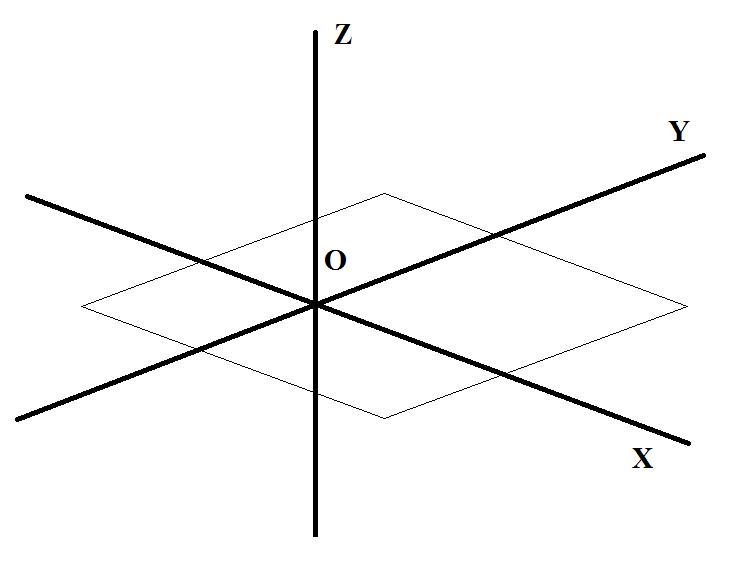
\includegraphics[width=0.5\textwidth]{abbildungen/01_ebene.png}
\caption{Ebene mit drei Geraden}
\label{fig:mathGrundl_einfuehrung_ebene}
\end{center}
\end{figure}
\"Uberdies sei auf jeder Gerade ein spezieller Punkt definiert: $I_{x}, I_{y}$ und $I_{z}$. Dieser Punkt habe vom Ursprung, entlang der jeweiligen Achse auf der er liegt, genau den Abstand 1. Man bezeichnet diesen Abstand als \textit{Einheitsl\"ange}. \newline
    Hinzukommend wird ein Vektor $\vect{e}_{x}$ definiert, welcher vom Ursprung aus auf den Punkt $I_{x}$ zeigt und damit zwangsl\"aufig auf der Geraden X liegt. Analog werden die Vektoren  $\vect{e}_{y}$ und $\vect{e}_{z}$ definiert. Diese Vektoren mit \textit{Einheitsl\"ange}, welche entlang der Koordinatenachsen liegen, werden \textit{Einheitsvektoren} genannt. Als Tripel notiert haben sie entlang der Achse, in welche  sie zeigen, eine 1 als Eintrag und sonst eine 0. Damit gilt $\vect{e}_{x}=\left( 1,0,0\right), \vect{e}_{y}=\left(0,1,0\right), \vect{e}_{z}=\left( 0,0,1\right)$. Durch die genannten Bedingungen ist es nicht m\"oglich einen der \textit{Einheitsvektoren} als \textit{Linearkombination} der anderen Beiden darzustellen. Damit bilden diese \textit{Einheitsvektoren} eine \textit{Basis} f\"ur einen \textit{Vektorraum} $V$. Da die \textit{Einheitsvektoren} genau drei unabh\"angige Vektoren sind, ist der von ihnen aufgespannte \textit{Vektorraum} gleich dem dreidimensionalen Raum. \newline
    Weiterhin sei ein Streckungsfaktor $\alpha \in \R$ definiert. Mit Hilfe von $\alpha \cdot I_{x}$ sei das Bild des Punktes $I_{x}$ beschrieben, welches sich durch Streckung mit Streckungszentrum im Ursprung $O$, entlang der x-Achse, um den Streckungsfaktor $\alpha$ ergibt. Die Zuordnung $\alpha \to \alpha \cdot I_{x}$ liefert damit eine eindeutige, umkehrbare Zuordnung der reellen Zahlen auf die Punkte der Geraden X. Dabei ist das Bild der Streckung des \textit{Einheitsvektors} $\vect{e}_{x}$ \"aquivalent mit dem Bild der Streckung des Punktes $I_{x}$. Zus\"atzlich seien f\"ur die Achsen Y und Z die Streckungsfaktoren $\beta$ und $\gamma$ nach dem gleichen Schema definiert. \newline
        
    Mit Hilfe dieser Festlegungen k\"onnen beliebige Punkte im Raum beschrieben werden. Alle Punkte des Raumes bilden dabei die \textit{Menge} $R^{3}$. Man sagt, dass die Punkte \textit{Elemente} dieser \textit{Menge} sind. Betrachtet man zum Beispiel einen Punkt auf der Ebene E, so kann man dieses \textit{Element} als Tripel von reellen Zahlen interpretieren: $P=\left( x_{1}, y_{1}, z_{1}\right)$. Man nennt dieses Tripel die \textit{Koordinaten} von $P$ (bez\"uglich des gew\"ahlten Koordinatensystems). Der Ursprung des Koordinatensystems hat bez\"uglich des Koordinatensystems, dessen Ursprung er ist, immer die Koordinaten $(0,0,0)$. Den Wert von $x_{1}$ erh\"alt man geometrisch durch Konstruktion einer Normalen bez\"uglich der x-Achse, welche den Punkt $P$ durchl\"auft. Den Fu\ss{}punkt dieser Normalen kann man durch Streckung des zuvor definierten Punktes $I_{x}$ um den Faktor $\alpha_{P}$ erhalten. Dabei entspricht eben diese reelle Zahl $\alpha_{P}$ dem Wert von $x_{1}$. \newline
    Die Werte f\"ur $y_{1}$ und $z_{1}$ ergeben sich analog. Die so erhaltene Zuordnung $P \to \left( x_{1}, y_{1}, z_{1}\right)$ bezeichnet man als eine Abbildung. Mit Hilfe dieser Abbildung wird beliebigen Punkten der Ebene E in eindeutiger Weise ein Zahlentripel von reellen Zahlen zugeordnet. Man sagt auch, dass dieses Zahlentripel ein \textit{Element} des \textit{Vektorraumes} $V$ ist, welcher \"uber dem \textit{K\"orper} der reellen Zahlen definiert ist. Aufgrund dessen, dass die Achsen des Koordinatensystems durch die \textit{Basis} des \textit{Vektorraumes} beschrieben werden, sind die Zahlenwerte des Tripels zwangsl\"aufig abh\"angig von der Wahl des Koordinatensystemursprungs und der \textit{Basisvektoren}. \newline
    Da dieses Zahlentripel nicht nur ein \textit{Element} einer \textit{Menge}, sondern insbesondere ein Vektor eines \textit{Vektorraumes} ist, gibt es alternative Schreibweisen f\"ur den Punkt $P$. Die \"Ublichste ist die Darstellung als Spaltenvektor $\vect{v} \in \R^{3}$. Dabei erh\"alt man $\vect{v}$ durch Subtraktion der Koordinaten des Punktes $P$ von den Koordinaten des gew\"ahlten Koordinatenursprungs. Beziehen sich alle Angaben auf das gleiche System, so entsprechen die Komponenten von $\vect{v}$ genau den Koordinaten von $P$ und die Darstellung als Spaltenvektor lautet: $\vect{v}=\begin{pmatrix} x_{1} \\ y_{1} \\ z_{1} \end{pmatrix}$. Man kann $\vect{v}$ auch als \textit{Linearkombination} der \textit{Basis} des \textit{Vektorraumes} $V$ darstellen: \begin{align*}
    \vect{v}&= x_{1} \vect{e}_{x} + y_{1} \vect{e}_{y} + z_{1} \vect{e}_{z} = \alpha_{P} \vect{e}_{x} + \beta_{P} \vect{e}_{y} + \gamma_{P} \vect{e}_{z}
\end{align*}      

  \begin{rem} Die Beschr\"ankung auf die Betrachtung von Rechtssystemen ist als einf\"uhrendes Beispiel besonders gut geeignet, da alle in dieser Arbeit verwendeten Koordinatensysteme die damit verbundenen Eigenschaften erf\"ullen sollen. Wollte man auch nicht orthogonale Koordinatensystem betrachten, so f\"uhrt dies zwangsl\"aufig auf die Betrachtung von kovarianten und kontravarianten Basisvektoren und die Tensorrechnung. Eine Einf\"uhrung in dieses Thema ist \cite{Roethlisberger2007} zu entnehmen. Eine ausf\"uhrliche Behandlung der Thematik ist in \cite{Jaenich2005} enthalten. 
  \end{rem}
  
   
  \section{Mengen}\label{sec:mathGrundl_mengen}
\begin{defn}[Mengen; nach G. Cantor] Eine Menge ist eine Zusammenfassung von bestimmten, wohlunterschiedenen Objekten unserer Anschauung oder unseres Denkens zu einem Ganzen. Die Objekte hei\ss{}en Elemente der Menge \cite{Cantor1895}. \newline
Ist $\set{M}$ eine Menge und $x$ ein Objekt, so notiert man $x \in \set{M}$, wenn die Menge $\set{M}$ das Objekt $x$ enth\"alt und $x \notin \set{M}$, wenn dies nicht der Fall ist. \newline
Enth\"alt die Menge $\set{M}$ keine Elemente, so nennt man dies die \textbf{leere Menge} \footnote{jede Menge besitzt die leere Menge als Teilmenge} $\lbrace  \rbrace$ beziehungsweise $\emptyset$.
\end{defn}
Mengen k\"onnen durch Aufz\"ahlung aller Elemente oder durch die Angabe von Eigenschaften, welche die Elemente erf\"ullen sollen, definiert werden. In Beispiel \ref{ex:mathGrundl_mengen} sind verschiedene Mengendefinition zu finden. \newline  
Die angegebene Definition f\"ur Mengen ist zwar anschaulich, verzichtet aber auf eine axiomatische Begr\"undung. Im Rahmen dieser Arbeit ist diese Definition jedoch ausreichend. Ein pr\"azise Definition von Mengen erfordert erheblichen Aufwand und ist beispielsweise in \cite{Asser1975} enthalten. \newline
  Die folgenden Mengen sind von besonderer Bedeutung: \begin{itemize}
  \item die nat\"urlichen Zahlen $\set{N}=\lbrace 0, 1, 2, \dots \rbrace$
  \item die ganzen Zahlen $\set{Z}=\lbrace 0, \pm 1, \pm 2, \dots \rbrace$
  \item die rationalen Zahlen $\set{Q}=\lbrace \left. \frac{p}{q} \right| q,p \in \set{Z}, q \neq 0 \rbrace$
  \item die reellen Zahlen $\set{R}$ als Menge aller, unter Umst\"anden nicht abbrechenden, Dezimalbr\"uche \cite[S. 12]{MatthiasPlaue2009}
  \end{itemize}

\begin{exmp}[Mengendefinitionen]\label{ex:mathGrundl_mengen} \begin{align*}
\set{M}_{1}&= \lbrace 1,2,5,8,10 \rbrace \\
\set{M}_{2}&= \lbrace x | x \text{ ist eine ganze Zahl und ungerade} \rbrace
\end{align*}
\end{exmp}  
  
  Die Reihenfolge der Elemente einer Menge ist ohne Bedeutung. Daher gilt $\set{M}_{1}= \lbrace 1,4,8 \rbrace = \lbrace 4,8,1 \rbrace $. Enth\"alt eine Menge ein Element mehrfach, so ist diese Multiplizit\"at ohne Bedeutung, daher gilt $\set{M}_{1}= \lbrace 1,3,5 \rbrace = \lbrace 1,3,5,3,5 \rbrace$. Zur Handhabung von Mengen gibt es eine Reihe von Axiomen, auf welche im Folgenden eingegangen wird. 

\subsection{Teilmengen} Es sei $\set{X}$ eine Menge und $P\of{x}$ eine Aussage. Die G\"ultigkeit der Aussage (wahr oder falsch) sei f\"ur alle Elemente $x$ \"uberpr\"ufbar. Man nennt dann \begin{align}
\set{Y}&= \lbrace \left. x\in \set{X}\right| P\of{x} \text{ ist wahr} \rbrace \label{gl:mathGrundl_mengen_teilmenge}
\end{align} eine \textbf{Teilmenge} von $\set{X}$ und notiert $\set{Y} \subset \set{X}$. \newline
 Die Mengen $\set{X}$ und $\set{Y}$ hei\ss{}en \textit{gleich}, wenn jedes Element von $\set{X}$ auch in $\set{Y}$ enthalten ist und umgekehrt: $\set{X}=\set{Y} \Leftrightarrow \forall x \left( x \in \set{X} \Leftrightarrow x \in \set{Y} \right)$. \newline
  Gilt $\set{Y} \subset \set{X} \land \set{Y} \neq \set{X}$, so nennt man $\set{Y}$ eine \textit{echte Teilmenge} von $\set{X}$ und notiert $\set{Y} \subsetneq \set{X}.$ \footnote{Mit dem Symbol $\land$ ist das logische Und - die \textit{Konjunktion} -  und mit dem Symbol $\lor$ ist das logische Oder - die \textit{Disjunktion} - gemeint. F\"ur Erkl\"arungen zu diesen logischen Operatoren siehe \cite[S. 28]{Arens2013}} \newline
  Die Gesamtheit aller Teilmengen einer Menge $\set{X}$ bildet die sogenannte \textbf{Potenzmenge} $\set{P}\of{\set{X}} = \lbrace \set{U}| \set{U} \subset \set{X} \rbrace $.  

\begin{rem}[Notation f\"ur Teilmengen] In der Literatur ist die Kennzeichnung einer echten Teilmenge im Gegensatz zu einer Teilmenge nicht einheitlich. Es gibt folgende Notationen: \begin{itemize}
\item Teilmenge: $\subset$, echte Teilmenge: $\subsetneq$
\item Teilmenge: $\subseteq$, echte Teilmenge: $\subset$
\end{itemize}
\end{rem}

  \subsection{Vereinigung und Durchschnitt}
  Sei $\set{X}$ eine Menge und $\set{I}$ eine Indexmenge, das hei\ss{}t die Elemente von $\set{I}$ sollen als Indizes dienen. Ist f\"ur jedes $i \in \set{I}$ eine Teilmenge $\set{X}_{i} \subset \set{X}$ gegeben, so nennt man  \begin{align}
  \underset{{i\in\set{I}}}{\bigcup} \set{X}_{i} &:= \lbrace \left. x \in \set{X} \right| \text{ es existiert ein } i \in \set{I} \text{ mit } x\in \set{X}_{i}\rbrace \label{gl:mathGrundl_mengen_vereinigung}
  \end{align}
  die \textbf{Vereinigung} der Mengen $\set{X}_{i}, i \in \set{I}$. In der so entstehenden Teilmenge von $\set{X}$ sind also all jene $x$ enthalten, die in wenigstens einer der vereinten  Teilmengen $\set{X}_{i}$ enthalten sind. \newline
  Der \textbf{Durchschnitt} \footnote{den \textit{Durchschnitt} von Mengen bezeichnet man auch kurz als \textit{Schnitt}} der Mengen wird mit 
  \begin{align}
  \underset{{i\in\set{I}}}{\bigcap} \set{X}_{i} &:= \lbrace \left. x \in \set{X} \right| x\in \set{X}_{i} \quad \forall  i \in \set{I} \rbrace \label{gl:mathGrundl_mengen_durchschnitt}
  \end{align}
  beschrieben. In der durch den Durchschnitt gebildeten Teilmenge von $\set{X}$ sind also diejenigen Elemente $x$ der Menge $\set{X}$ enthalten, welche in allen Teilmengen $\set{X}_{i}$ enthalten sind, von denen der Durchschnitt gebildet wurde. \newline
  F\"ur die Verkn\"upfung von zwei Mengen schreibt man insbesondere: \begin{align*}
  \set{X}_{1} \cup \set{X}_{2} &= \lbrace \left. x \right| x \in \set{X}_{1} \lor x \in \set{X}_{2} \rbrace
  \end{align*}
  f\"ur die Vereinigung und \begin{align*}
  \set{X}_{1} \cap \set{X}_{2} &= \lbrace \left. x \right| x \in \set{X}_{1} \land x \in \set{X}_{2} \rbrace
  \end{align*}
  f\"ur den Durchschnitt. \newline
  Ist der Durchschnitt zweier Mengen leer, gilt also \begin{align}
  \set{X}_{1} \cap \set{X}_{2} = \emptyset \label{gl:mathGrundl_mengen_disjunkt}
\end{align} dann bezeichnet man die Mengen als \textbf{disjunkt}.

  \subsection{Differenz von Mengen} Sind $\set{X}_{1}$ und $\set{X}_{2}$ Teilmengen einer Menge $\set{X}$, so hei\ss{}t \begin{align}
  \set{X}_{1} - \set{X}_{2} &:= \lbrace \left.x \in \set{X}_{1}\right| x \notin \set{X}_{2} \rbrace \label{gl:mathGrundl_mengen_differenz}
  \end{align}
  die \textbf{Differenz} von $\set{X}_{1}$ und $\set{X}_{2}$. Auch dies ist eine Teilmenge von $\set{X}$ und sogar von $\set{X}_{1}$.
  
  
  \subsection{Kartesisches Produkt}
   Es seien $\set{X}_{1}, \dots, \set{X}_{n}$ Mengen. Dann hei\ss{}t \begin{align}
  \underset{i=1}{\overset{n}{\prod}}&= \lbrace \left.\left( x_{1}, \dots, x_{n} \right)\right| x_{1} \in \set{X}_{1}, \dots, x_{n} \in \set{X}_{n}  \rbrace \label{gl:mathGrundl_mengen_kartProd}
  \end{align}
  das \textbf{kartesische Produkt} der Mengen $\set{X}_{1}, \dots, \set{X}_{n}$. Eine gleichbedeutende Notation lautet $\set{X}_{1} \times \dots \times \set{X}_{n}$. Die Elemente $\left( x_{1}, \dots, x_{n} \right)$ werden als \textbf{n-Tupel} mit Komponenten $x_{i} \in \set{X}_{i}, i=1, \dots, n$, bezeichnet. \newline
  Zwei n-Tupel $\left( x_{1}, \dots, x_{n} \right), \left( x'_{1}, \dots, x'_{n} \right)$ gelten genau dann als gleich, wenn $x_{i}=x'_{i}$ f\"ur $i=1, \dots, n$ erf\"ullt ist. \newline
  Das 2-Tupel $(3, 5)$ beschreibt einen Punkt auf einer Zahlenebene. Ein Tupel, welche genau zwei Elemente beinhaltet, bezeichnet man als \textit{Paar}. \newline  
  Ein 3-Tupel bezeichnet man als \textit{Tripel}. Ein Beispiel f\"ur ein Tripel ist der K\"orper $\left( \set{R}, +, \cdot \right)$, welcher durch die Menge der reellen Zahlen $\set{R}$ mit den Verkn\"upfungen Addition und Multiplikation gebildet wird. 

  \subsection{M\"achtigkeit}
   Sei $\set{X}$ eine Menge, dann bezeichnet man mit \begin{align}
  \abs{\set{X}} \label{gl:mathGrundl_mengen_maechtigkeit}
  \end{align} die \textbf{M\"achtigkeit} der Menge und meint damit die Anzahl der Elemente, welche in $\set{X}$ enthalten sind. Es gilt \begin{align*}
  \abs{\set{X}} &:= \begin{cases}n, \text{ falls $\set{X}$ endlich ist und $n$ Elemente enth\"alt} \\ \infty, \text{ falls $\set{X}$ nicht endlich ist.} \end{cases}
\end{align*}   

%  \subsection{Rechengesetze f\"ur Mengen} Kommutativit\"at usw. 
%  siehe \cite[S.14]{MatthiasPlaue2009}
  
  \section{Abbildung}\label{sec:mathGrundl_abbildung}
  \begin{defn}[Abbildung] Eine Abbildung $f: \set{X} \longrightarrow \set{Y}$ zwischen zwei Mengen $\set{X}$ und $\set{Y}$ ist eine Vorschrift, welche jedem $x \in \set{X}$ ein wohlbestimmtes Element $y \in \set{Y}$ zuordnet, welches mit $f\of{x}$ bezeichnet wird. Man schreibt auch \hfill \newline
   $x \longmapsto f\of{x}$. Man bezeichnet $\set{X}$ als den Definitionsbereich und $\set{Y}$ als den Bild- \footnote{der Bildbereich wird auch Zielmenge genannt} oder Wertebereich  der Abbildung $f$.
  \end{defn}
  \subsection{Komposition von Abbildungen}
  Gegeben seien zwei Abbildungen $f: \set{X} \longrightarrow \set{Y}$ und $g: \set{Y} \longrightarrow \set{Z}$ zwischen Mengen. Dann kann man die Abbildungen komponieren: \begin{align}
  g \circ f &: \set{X} \longrightarrow \set{Z}, &x&\longmapsto g\of{f\of{x}}. \label{gl:mathGrundl_abbildung_komposition}
  \end{align}
  Alternative Bezeichnungen f\"ur eine Komposition lauten \textit{Hintereinanderausf\"uhrung} und \textit{Verkettung}.
  
  \begin{exmp}[Ort als Bild der Zeit] Ordnet man jedem Zeitpunkt $t$ den Ort beziehungsweise die Position des Schwerpunkts eines K\"orpers zu, so entspricht dies einer Abbildung $f: t \longmapsto f\of{t}$ Der Definitionsbereich sei beispielsweise gegeben durch beliebige positive reelle Zahlen und der Wertebereich durch beliebige reelle Zahlen. Der K\"orper kann sich dann frei im Anschauungsraum bewegen und seine Position ist mit Hilfe der Abbildung $f\of{t}$ eindeutig beschrieben. 
  \end{exmp}
  
  \begin{rem}[Umkehrbarkeit einer Abbildung] In der Definition einer Abbildung wird gefordert, dass jedem $x \in \set{X}$ ein eindeutiges Bild $y \in \set{Y}$ zugeordnet wird. Die Umkehrung, dass jedem $y \in \set{Y}$ ein eindeutiges Urbild $x \in \set{X}$ zugeordnet werden kann, kann daraus nicht geschlussfolgert werden.
  \end{rem}
  
  Seien $\set{M}\subset \set{X}, \set{N}\subset \set{Y}$ und $f: \set{X}\longrightarrow\set{Y}$ eine Abbildung, so nennt man: \begin{align}
  f\of{\set{M}}&:= \lbrace \left.y\in\set{Y}\right| \text{ es existiert ein } x\in\set{M} \text{ mit } y=f\of{x} \rbrace \label{gl:mathGrundl_abbildung_bild}
  \end{align} \textbf{Bild}(-menge) von $\set{M}$ unter der Abbildung $f$ und \begin{align}
  f^{-1}\of{\set{N}}&:= \lbrace \left.x\in\set{X}\right| f\of{x}\in \set{N} \rbrace \label{gl:mathGrundl_abbildung_urbild}
  \end{align} \textbf{Urbild}(-menge) von $\set{N}$ unter der Abbildung $f$. \newline
  Weiterhin bezeichnet man $f$ als 
  \begin{itemize}
  \item \textbf{injektiv}, falls f\"ur $x_{1},x_{2}\in \set{X}$ gilt: $f\of{x_{1}}=f\of{x_{2}}\implies x_{1}=x_{2}$, das hei\ss{}t, dass verschiedene Elemente des Definitionsbereichs auf verschiedene Elemente des Wertebereichs abgebildet werden beziehungsweise dass das Urbild $f^{-1}\of{y}$ eines jeden $y\in\set{Y}$ entweder leer ist, oder aus genau einem $x\in\set{X}$ besteht
  \item \textbf{surjektiv}, falls gilt: $\forall y \in \set{Y} \quad \exists x \in\set{X}: f\of{x}=y$  , das hei\ss{}t jedes Element des Wertebereichs wird durch Abbildung mindestens eines Elements aus dem Definitionsbereich erreicht
  \item \textbf{bijektiv}, falls $f$ injektiv und surjektiv ist. F\"ur bijektive Abbildungen $f$ l\"asst sich die \textbf{Umkehrabbildung} $g: \set{Y}\longrightarrow \set{X}, g:=f^{-1}$ bilden, welche jedem Element der Bildmenge ein Element aus dem Definitionsbereich zuordnet. 
  \end{itemize}
  \begin{defn}[Lineare Abbildung]  Eine Abbildung $f:\set{V}\longrightarrow \set{V}'$ zwischen den Vektorr\"aumen $\set{V}, \set{V}'$ \"uber dem K\"orper $\set{K}$ hei\ss{}t lineare Abbildung \"uber $\set{K}$, falls gilt: \begin{align}
  f\of{a+b}&= f\of{a}+f\of{b} \text{ f\"ur } a,b \in \set{V} \\\label{gl:mathGrundl_abbildung_linAbb_add}
  f\of{\alpha a}&= \alpha f\of{a} \text{ f\"ur } \alpha \in \set{K}, a\in \set{V}.
  \end{align} Daraus folgen die notwendigen Rechenregeln \begin{align*}
  f\of{0}&=0 \\
  f\of{-a}&= -f\of{a} \text{ f\"ur } a \in \set{V}. 
  \end{align*}
  \end{defn}
  
%  \subsection{Eigenschaften von Abbildungen}
%  siehe \cite{Modler2011d}, insbesondere f\"ur \textit{Kompositionen} \cite[S. 37]{MatthiasPlaue2009}
    
  
   \section{Gruppen}\label{sec:mathGrundl_gruppen}
  Unter einer \textbf{inneren Verkn\"upfung} auf einer Menge $\set{M}$ versteht man eine Abbildung $f: \set{M} \times \set{M} \to \set{M}$. Sie ordnet jedem Paar $(a, b)$ von Elementen aus $\set{M}$ ein Element $f(a, b) \in \set{M}$ zu. Die innere Verkn\"upfung muss also eine abgeschlossene \footnote{der Begriff \textit{Abgeschlossenheit} wird im Abschnitt \ref{sec:mathGrundl_koerper} genauer erkl\"art} Verkn\"upfung sein. Es wird die Notation $ a \cdot b$ anstelle von $f\of{a,b}$ verwendet, um den verkn\"upfenden Charakter der Abbildung zu verdeutlichen. \newline
  Ist die Verkn\"upfung kommutativ, gilt also $f\of{a,b}=f\of{b,a}$ f\"ur alle $a,b \in \set{M}$, so wird die Verkn\"upfung $f$ durch $a+b$ notiert. 
  
  \begin{defn} Eine Menge $\set{G}$ mit einer inneren Verkn\"upfung $\circ: \set{G} \times \set{G} \longrightarrow \set{G},$ \hfill \newline  $(a, b) \longmapsto a \circ b$, hei\ss{}t eine Gruppe $\of{\set{G}, \circ}$, wenn die folgenden Eigenschaften erf\"ullt
sind:
\begin{itemize}
\item Die Verkn\"upfung $\circ$ ist assoziativ, d. h. es gilt \begin{align}
(a \circ b) \circ c &= a \circ (b \circ c) \quad \forall { } a, b, c \in \set{G}. \label{gl:mathGrundl_gruppen_assoziativ}
\end{align}
\item Es existiert ein \textbf{neutrales Element} $e$ in $\set{G}$, das hei\ss{}t ein Element $e \in \set{G}$ mit \begin{align}
e \circ a = a \circ e = a \quad \forall { } a \in \set{G}. \label{gl:mathGrundl_gruppen_neutrElem}
\end{align} Das neutrale Element einer Gruppe ist offensichtlich zugleich links-neutral und rechts-neutral.
\item Zu jedem $a \in \set{G}$ gibt es ein \textbf{inverses Element}, das hei\ss{}t ein Element $b \in \set{G}$ mit \begin{align}
a \circ  b = b \circ  a = e. \label{gl:mathGrundl_gruppen_invElemt}
\end{align} Dabei ist $e$ das nach \eqnref{gl:mathGrundl_gruppen_neutrElem} existierende (eindeutig bestimmte) neutrale Element von $\set{G}$. Das inverse Element $b$ einer Gruppe ist links-invers und recht-invers.
\item Die Gruppe $\of{\set{G}, \circ}$ hei\ss{}t kommutativ oder \textbf{abelsch}, falls die Verkn\"upfung kommutativ ist, das hei\ss{}t falls zus\"atzlich gilt: \begin{align}
a \circ b = b \circ a \quad \forall { } a, b \in \set{G}. \label{gl:mathGrundl_gruppen_kommutativ}
\end{align}
\end{itemize}
  \end{defn}  
  \begin{exmp}[Beispiele f\"ur Gruppen]\hfill \newline
  \begin{itemize}
  \item Die Menge $\set{Z}$ mit der Verkn\"upfung Addition \glqq $+$\grqq { }
  \item Die Menge $\set{R}$ mit der Verkn\"upfung Addition \glqq $+$\grqq { } und $\set{R}^{\ast}:=\set{R}-\lbrace 0 \rbrace $ mit der Multiplikation \glqq$\cdot$\grqq { }
  \end{itemize}
  
\end{exmp}    
  
  \begin{rem}[multiplikative Verkn\"upfungen] Ist die Verkn\"upfung einer Gruppe in multiplikativer Schreibweise gegeben, so wird \begin{itemize}
  \item das neutrale Element $e$ als \textbf{Einselement} bezeichnet und als 1 notiert
  \item das inverse Element $b$ zu $a$ als $a^{-1}$ notiert
  \item das Verkn\"upfungszeichen \glqq$\cdot$\grqq { }meist weggelassen
  \item f\"ur endliche Elemente $a_{1}, \dots, a_{n}\in\set{G}$ das Produkt der Elemente als \hfill \newline $\underset{i=1}{\overset{n}{\prod}}a_{i}:=a_{1} \cdot \dots \cdot a_{n}$ definiert, wobei $\underset{i=1}{\overset{0}{\prod}}a_{i}:= 1$ gilt.
  \end{itemize}
\end{rem}    

\begin{rem}[additive Verkn\"upfungen] Ist die Verkn\"upfung einer Gruppe kommutativ, so verwendet man die additive Schreibweise und \begin{itemize}
  \item bezeichnet das neutrale Element $e$ als \textbf{Nullelement} und schreibt 0
  \item notiert das inverse Element $b$ zu $a$ als $-a$
  \item definiert f\"ur endliche Elemente $a_{1}, \dots, a_{n}\in\set{G}$ die Summe der Elemente als \hfill \newline $\underset{i=1}{\overset{n}{\sum}}a_{i}:=a_{1} + \dots + a_{n}$, wobei $\underset{i=1}{\overset{0}{\sum}}a_{i}:= 0$ gilt.
  \end{itemize}
\end{rem} 
  
  \section{K\"orper}\label{sec:mathGrundl_koerper}
  K\"orper sind Zahlsysteme mit gewissen Axiomen f\"ur die Addition und Multiplikation, welche auf den Axiomen von Gruppen aufbauen. \newline
  \begin{defn}[K\"orper]\label{def:mathGrundl_koerper} Ein K\"orper ist eine Menge $\set{K}$ mit zwei inneren Verkn\"upfungen, geschrieben als Addition und Multiplikation, so dass folgende Bedingungen erf\"ullt sind: \begin{enumerate}
  \item $\set{K}$ ist eine abelsche Gruppe bez\"uglich der Addition, das hei\ss{}t die Addition ist assoziativ nach \eqnref{gl:mathGrundl_gruppen_assoziativ}, hat ein neutrales Element 0 nach \eqnref{gl:mathGrundl_gruppen_neutrElem} und ein inverses Element $-a\in \set{K}$ nach \eqnref{gl:mathGrundl_gruppen_invElemt} zu $a\in\set{K}$ und sie ist kommutativ nach \eqnref{gl:mathGrundl_gruppen_kommutativ}
  \item $\set{K}^{\ast}=K\backslash \lbrace 0 \rbrace$ ist eine abelsche Gruppe bez\"uglich der Multiplikation, das hei\ss{}t die Multiplikation ist assoziativ nach \eqnref{gl:mathGrundl_gruppen_assoziativ}, hat das neutrale Element 1 nach \eqnref{gl:mathGrundl_gruppen_neutrElem} und das inverse Element $a^{-1}$ nach \eqnref{gl:mathGrundl_gruppen_invElemt} f\"ur $a, a^{-1} \in \set{K}$ und sie ist kommutativ nach \eqnref{gl:mathGrundl_gruppen_kommutativ}
  \item Es gelten die Distributivgesetze: \begin{align*}
  a \cdot \left( b + c \right) &= a \cdot b + a \cdot c \\
  \left( a + b \right) \cdot c &= a\cdot c + b \cdot c 
  \end{align*} f\"ur $a,b,c \in \set{K}$
  \end{enumerate}
  Wird ein K\"orper mit den zugeh\"origen Verkn\"upfungen angegeben, so kann man $\set{K}$ als Tripel $\left(\set{K}, +, \cdot \right) $ notieren.
  \end{defn}
  \begin{rem}[Abgeschlossenheit] Entsprechend der Definition \ref{def:mathGrundl_koerper} f\"ur einen K\"orper $\set{K}$ bilden die Rechenoperationen Addition und Multiplikation Elemente des K\"orpers auf Elemente des K\"orpers ab. Da $\set{K}$ nie verlassen wird, spricht man in diesem Zusammenhang von der \textbf{Abgeschlossenheit} des K\"orpers $\set{K}$.
\end{rem} 
\begin{rem}[K\"orper und Gruppen] Ist $\set{K}$ ein K\"orper mit den Verkn\"upfungen Addition und Multiplikation, dann sind $\left(\set{K}, + \right)$ und $\left(\set{K} - \lbrace 0 \rbrace, \cdot \right)$ Gruppen. \newline
Die Menge aller invertierbaren $n \times n$ Matrizen \"uber einem K\"orper mit Matrizenmultiplikation bildet die \textit{allgemeine lineare Gruppe}.
\end{rem}
   
 \begin{exmp}[K\"orper] H\"aufig verwendete K\"orper sind \begin{itemize}
 \item die Menge der rationalen Zahlen $\set{Q}$ mit den Verkn\"upfungen Addition und Multiplikation
 \item  die Menge der reellen Zahlen $\set{R}$ mit den Verkn\"upfungen Addition und Multiplikation
 \item die Menge $\set{R}\times \set{R}:= \lbrace \left.(x, y)\right| x,y \in \set{R} \rbrace$ der Paare (2-Tupel) reeller Zahlen mit den Verkn\"upfungen Addition und Multiplikation. Mit den Verkn\"upfungen \begin{align*}
 \left( x_{1}, y_{1}\right)+ \left( x_{2}, y_{2}\right)&= \left( x_{1}+x_{2}, y_{1}+y_{2}\right)\\
 \left( x_{1}, y_{1}\right) \cdot \left( x_{2}, y_{2}\right)&= \left( x_{1}x_{2}-y_{1}y_{2}, x_{1}y_{2}+x_{2}y_{1}\right)\\
 \end{align*} und den neutralen Elementen der Addition: $(0,0)$ und Multiplikation: $(1,0)$ bildet diese Menge einen K\"orper. Jedes Zahlenpaar $\left(x, y \right)$ kann als Linearkombination dargestellt werden: \begin{align*}
 \left(x, y \right) &= x \cdot \left( 1,0 \right) + y \cdot \left( 0, 1 \right).
\end{align*} F\"uhrt man folgende Schreibweisen ein: \begin{itemize}
\item $\left( 1,0 \right): 1$
\item $\left( 0,1 \right): i$ und bezeichnet $i$ als imagin\"are Einheit,
\end{itemize} so erh\"alt man die Darstellung $\left(x, y \right) \equiv x + i y$. Die so erhaltenen, reellen Zahlenpaare bezeichnet man als die \textbf{komplexen Zahlen}, welche in \textit{algebraischer Normalform} vorliegen. Der K\"orper der komplexen Zahlen lautet damit $\left(\set{C},+,\cdot \right)$.
 \end{itemize}
 Die Menge der nat\"urlichen Zahlen $\set{N}$ bildet mit der Addition \textit{keinen} K\"orper, denn es gibt kein inverses Element bez\"uglich der Addition. F\"ur das Element $5$ ist beispielsweise das zu erwartende, inverse Element $-5$ offensichtlich $-5\notin \set{N}$. \newline
 Die Menge der ganzen Zahlen $\set{Z}$ bildet mit der Addition zwar eine abelsche Gruppe aber keinen K\"orper, denn es gibt kein inverses Element bez\"uglich der Multiplikation. Das Element $a=8\in\set{Z}$ hat zum Beispiel kein inverses Element $b=1\cdot a^{-1}$ f\"ur welches $b\in\set{Z}$ gilt.   
 \end{exmp}
  
%  \subsection{Weitere Eigenschaften und Begriffe}
%  insbesondere Homomorphismen f\"ur Gruppen und K\"orper \cite[S. 86, 87, 89, 93]{Modler2011d} \hfill \newline
%  Kern und Bild eines Homomorphismus \cite[S. 86, 93!]{Modler2011d}
  
  \section{Vektorr\"aume}\label{sec:mathGrundl_vektorraeume}
  Ein Vektorraum ist durch eine abelsche Gruppe mit der inneren Verkn\"upfung Addition $\left(\set{V}, +\right)$ (Abschnitt \ref{sec:mathGrundl_gruppen}), einen K\"orper $\set{K}$ (Abschnitt \ref{sec:mathGrundl_koerper}) mit Skalaren als Elementen, eine \"au\ss{}ere Multiplikation, welche Elemente von $\set{K}$ mit denen von $\set{V}$ verkn\"upft und auf $\set{V}$ abbildet, und vier Vertr\"aglichkeitsgesetzen - den so genannten Vektorraumaxiomen -  gegeben. Der K\"orper $\set{K}$ entspricht h\"aufig den reellen Zahlen $\set{R}$ oder den komplexen Zahlen $\set{C}$. 
  \begin{defn}[$\set{K}-$Vektorraum]\label{def:mathGrundl_vektorraeume_vektorraum} Es sei $\set{K}$ ein K\"orper, $\left(\set{V}, +\right)$ eine abelsche Gruppe und \begin{align}
  \cdot : & \set{K}\times \set{V} \longrightarrow V, &\left( \lambda, \vect{x}\right) &\longmapsto \lambda \cdot \vect{x}
  \end{align}
  eine Abbildung. Ferner seien die Vektoren $\vect{x},\vect{y},\vect{z}\in \set{V}$ und die Skalare $\lambda, \mu \in \set{K}$ gegeben. Man nennt $\set{V}$ einen Vektorraum \"uber dem K\"orper $\set{K}$ oder kurz einen $\set{K}-$Vektorraum genau dann, wenn die folgenden Eigenschaften erf\"ullt sind: \begin{align}
  \intertext{Assoziativit\"at der Multiplikation mit Skalaren} 
  \left( \lambda \mu \right)\cdot \vect{x}&= \lambda \cdot \left( \mu \cdot \vect{x} \right)\label{gl:mathGrundl_vektorraeume_assoz}\\
  \intertext{Distributivit\"at}   
  \lambda \cdot \left( \vect{x}+\vect{y} \right)&=\lambda \cdot \vect{x} + \lambda \cdot \vect{y} \label{gl:mathGrundl_vektorraeume_distr1} \\
  \intertext{und} 
  \left( \lambda + \mu \right) \cdot \vect{x} &= \lambda \cdot \vect{x}+ \mu \cdot \vect{x} \label{gl:mathGrundl_vektorraeume_distr2}  \\
  \intertext{F\"ur die Multiplikation gibt es ein neutrales 1-Element}
  1\cdot \vect{x}&= \vect{x} \label{gl:mathGrundl_vektorraeume_neutrElem}  
  \end{align}
  \end{defn}
  Die Vektorraumaxiome nach \eqnref{gl:mathGrundl_vektorraeume_assoz} - \eqnref{gl:mathGrundl_vektorraeume_neutrElem} beschreiben eine Vertr\"aglichkeit der zwei Verkn\"upfungen Addition und Multiplikation des $\set{K}-$Vektorraums. \hfill \newline 
    Die Elemente eines Vektorraumes werden als \textbf{Vektoren} bezeichnet. Vektoren werden allein durch ihre Eigenschaften definiert. Typische Beispiele f\"ur Vektoren sind Elemente der  Vektorr\"aume $\set{R}^{2}$ und $\set{R}^{3}$, aber auch Funktionen k\"onnen Vektoren sein. Ein Vektor ist also nicht zwangsl\"aufig ein Pfeil mit L\"ange und Richtung. \hfill \newline
  Das neutrale Element der Addition der abelschen Gruppe $\set{V}$ wird als Nullvektor bezeichnet und mit $\vect{0}$ gekennzeichnet. Ist aus dem Kontext erkennbar, dass es sich um einen Nullvektor handelt, so wird die besondere Notation als Vektor h\"aufig weggelassen und man schreibt $0$ f\"ur den Nullvektor. 
 \begin{rem}[unendliche Vektorr\"aume] F\"ur jeden K\"orper $\set{K}$ und jede nat\"urliche Zahl $n$ ist die Menge \begin{align*}
 \set{V}&=\set{K}^{n} = \left\lbrace \left.\begin{pmatrix}
 v_{1} \\ \vdots \\ v_{n}
\end{pmatrix} \right| v_{1}, \dots, v_{n} \in \set{K}  \right\rbrace
 \end{align*} mit komponentenweiser Addition und Multiplikation mit Skalaren aus $\set{K}$ ein $\set{K}-$Vektorraum. Insbesondere werden somit f\"ur den K\"orper der reellen Zahlen $\set{R}$ der reelle Vektorraum $\set{R}^{n}$ und f\"ur den K\"orper der komplexen Zahlen $\set{C}$ der komplexe Vektorraum $\set{C}^{n}$ definiert. 
 \end{rem}
  
 
  
  \begin{defn}[Untervektorraum] Sei $\set{V}$ ein $\set{K}-$Vektorraum. Eine Teilmenge $\set{U}\subset \set{V}$ hei\ss{}t ein $\set{K}-$Untervektorraum oder \textbf{linearer Unterraum von} $\mathbf{\set{V}}$, wenn gilt: \begin{align}
  \set{U}&\neq \emptyset \label{gl:mathGrundl_vektorraeume_unterRaum_nichtLeer} \\
  \vect{a}, \vect{b} \in \set{U}&\implies \vect{a}+ \vect{b} \in \set{U} \label{gl:mathGrundl_vektorraeume_unterRaum_addition} \\
  \alpha \in \set{K}, \vect{a}\in \set{U} &\implies \alpha \vect{a} \in \set{U} \label{gl:mathGrundl_vektorraeume_unterRaum_skalarMult}
  \end{align}
  \end{defn}
  \begin{rem}[Untervektorraum] Ein Untervektorraum enth\"alt in jedem Fall den Nullvektor. Au\ss{}erdem ist ein Untervektorraum bez\"uglich der Addition und der Multiplikation mit Skalaren abgeschlossen. Ein Untervektorraum von einem Vektorraum ist stets selbst ein Vektorraum.
  \end{rem}

  \begin{defn}[Linearkombination]\label{def:mathGrundl_vektorraeume_linearKombi} Sei $\set{V}$ ein $\set{K}-$Vektorraum. Ein beliebiger Vektor $\vect{v}\in\set{V}$ hei\ss{}t \textbf{Linearkombination} einer Anzahl von Vektoren $\vect{v}_{1},\dots,\vect{v}_{k} \in \set{V}$, falls Skalare $\lambda_{1},\dots,\lambda_{k}\in\set{K}$ derart existieren, dass \begin{align*}
  \vect{v}&=\sum_{i=1}^{k} \lambda_{i} \vect{v}_{i}
  \end{align*}
  erf\"ullt ist. Der Vektor $\vect{v}$ l\"asst sich dann aus den Vektoren $\vect{v}_{1},\dots,\vect{v}_{k}$ mit den \textit{Koeffizienten} $\lambda_{1},\dots,\lambda_{k}$ \textit{linear kombinieren}. Eine \"aquivalente Aussage w\"are, dass der Vektor $\vect{v}$ von den Vektoren $\vect{v}_{1},\dots,\vect{v}_{k}$ \textit{linear abh\"angig} ist. 
  \end{defn}
  
  \begin{defn}[Spann, Lineare H\"ulle] Sei $\set{V}$ ein $\set{K}-$Vektorraum. Die Menge aller m\"oglichen Linearkombinationen einer gegebenen Menge von Vektoren $\vect{v}_{1},\dots,\vect{v}_{k}\in\set{V}$ wird als \textbf{Spann} oder die \textbf{lineare H\"ulle} dieser Vektoren bezeichnet: \begin{align}
  \Span\left\lbrace \vect{v}_{1},\dots,\vect{v}_{k}\right\rbrace&= \left\lbrace \left. v=\sum_{i=1}^{k} \lambda_{i}\vect{v}_{i}\right| \lambda_{i}\in\set{K} \right\rbrace \label{gl:mathGrundl_vektorraeume_span}
  \end{align}
  \end{defn}
  
  \begin{defn}[Erzeugendensystem] Eine Anzahl von Vektoren $\vect{v}_{1},\dots,\vect{v}_{k}\in\set{V}$ eines $\set{K}-$Vektorraumes $\set{V}$ hei\ss{}t \textbf{Erzeugendensystem} von $\set{V}$, wenn gilt: \begin{align}
  \Span\left\lbrace \vect{v}_{1},\dots,\vect{v}_{k}\right\rbrace&= \set{V} \label{gl:mathGrundl_vektorraeume_erzeugSys}
  \end{align} Es l\"asst sich also jeder Vektor des $\set{K}-$Vektorraumes $\set{V}$ durch Linearkombination eines zugeh\"origen Erzeugendensystems darstellen. Ist die M\"achtigkeit des Erzeugendensystems endlich, so ist $\set{V}$ \textit{endlich erzeugt}. \newline
  Jedes Erzeugendensystem eines endlichen Vektorraumes $\set{V}$ enth\"alt eine \textbf{Basis}.
  \end{defn}
  \begin{rem}[Erzeugendensystem f\"ur $\set{R}^{n}$]\label{rem:mathGrundl_vektorraeume_kanBasis} Jeder Vektorraum $\set{V}$, der \"uber dem K\"orper der reellen Zahlen $\set{R}$ definiert wird, besitzt ein Erzeugendensystem. \hfill \newline
  Im $\set{R}-$ Vektorraum $\set{R}^{n}$ bilden die \textit{Einheitsvektoren} $\vect{e}_{1},\dots,\vect{e}_{n}$ ein Erzeugendsystem. Ein Einheitsvektor $\vect{e}_{i}$ hat in der i-ten Zeile eine eins als Eintrag. Alle weiteren Eintr\"age dieses Einheitsvektors sind null. \begin{align*}
  \vect{e}_{i}&=\begin{pmatrix}
  0 \\ 
  \vdots \\ 
  0 \\ 
  1 \\ 
  0 \\
  \vdots \\
  0
  \end{pmatrix} \leftarrow \text{ i-te Zeile }
  \end{align*}
  Ein solches Erzeugendensystem wird als \textit{kanonische Basis} bezeichnet.
  \end{rem}
  
  \begin{defn}[Lineare Unabh\"angigkeit] Eine Menge von Vektoren \hfill \newline
  $\lbrace \vect{v}_{1},\dots,\vect{v}_{n} \rbrace$ eines $\set{K}-$Vektorraums $\set{V}$ hei\ss{}t \textbf{linear unabh\"angig}, wenn sich keiner der Vektoren $\vect{v}_{1},\dots,\vect{v}_{n}$ als Linearkombination der \"Ubrigen darstellen l\"asst. Die Gleichung
  \begin{align}
  \sum_{i=1}^{n} \lambda_{i}\vect{v}_{i}&=\vect{0} \label{gl:mathGrundl_vektorraeume_linUnabh}
  \end{align}
  mit den Koeffizienten $\lambda_{i}\in\set{K}$ besitzt also nur die triviale L\"osung $\lambda_{1},\dots,\lambda_{n}=0$. Es gilt also \begin{align*}
  \sum_{i=1}^{n} \lambda_{i}\vect{v}_{i}&=\vect{0} \implies \lambda_{i}=0 \quad \forall i.
\end{align*}   \hfill \newline
  Eine nicht linear unabh\"angige Menge hei\ss{}t \textbf{linear abh\"angig}. Bei einer linear abh\"angigen Menge gibt es nicht triviale L\"osungen der \eqnref{gl:mathGrundl_vektorraeume_linUnabh} und damit nicht triviale Darstellungen des Nullvektors. Es existieren also $\lambda$ mit $\lambda\neq 0$, so dass gilt $\vect{v}_{i}=\lambda \vect{v}_{j}$. Die Vektoren $\vect{v}_{i}, \vect{v}_{j}$ sind dann Vielfache voneinander beziehungsweise parallel zueinander.
\end{defn}   
  \begin{rem}[Lineare Abh\"angigkeit] Eine linear unabh\"angige Menge ist unverk\"urzbar. Werden Vektoren aus dieser Menge entfernt, so spannt die Menge weniger Raum auf. \hfill \newline
  Bei einer linear abh\"angigen Menge liegt wenigstens einer der Vektoren in der linearen H\"ulle der Anderen. Er kann daher weggelassen werden, ohne die H\"ulle zu verkleinern. 
\end{rem}   
  
  \begin{defn}[Basis]\label{def:mathGrundl_vektorraeume_basis} Gegeben sei ein $\set{K}-$Vektorraum $\set{V}$. Ein System von Vektoren $\vect{v}_{1},\dots,\vect{v}_{n}$ von $\set{V}$ wird als \textbf{Basis} von $\set{V}$ bezeichnet, wenn gilt: \begin{enumerate}
  \item Die Vektoren $\vect{v}_{1},\dots,\vect{v}_{n}$ bilden ein Erzeugendensystem von $\set{V}$, es gilt also $\Span\lbrace \vect{v}_{1},\dots,\vect{v}_{n} \rbrace=\set{V}$.
  \item Das System $\vect{v}_{1},\dots,\vect{v}_{n}$ ist linear unabh\"angig. Die Basis ist daher unverk\"urzbar. 
\end{enumerate}
  Die Anzahl der Elemente einer Basis eines Vektorraumes $\set{V}$ wird als \textbf{Dimension} des Vektorraumes bezeichnet: $\dim \set{V}$.
  \end{defn}

 \subsection{Matrizen}\label{ssec:mathGrundl_vektorraeume_matrizen}
  Es seien $m$ und $n$ nat\"urliche Zahlen. Eine $m\times n$ Matrix $\matr{A}$ \"uber dem K\"orper $\set{K}$ ist eine Abbildung \begin{align*}
  \matr{A}:& \begin{cases} \lbrace 1, \dots, m \rbrace \times \lbrace 1,\dots,n \rbrace \longrightarrow \set{K}, \\
  \left( i, j\right) \longmapsto a_{ij}.
  \end{cases}
  \end{align*}
  Dabei bezeichnet $i$ den Zeilenindex und $j$ den Spaltenindex. Die K\"orperelemente $a_{ij}\in \set{K}, i=1, \dots, m, j=1, \dots, n$ nennt man \textbf{Komponenten} oder die \textbf{Eintr\"age} der Matrix $\matr{A}$. Eine Matrix $\matr{A}$ kann \"ubersichtlich durch $m$ Zeilen und $n$ Spalten dargestellt werden: \begin{align*}
  \matr{A}&=\begin{pmatrix}
  a_{11} & a_{12} & \dots & a_{1n} \\
  a_{21} & a_{22} & \dots & a_{2n} \\
  \vdots & \vdots & \dots & \vdots \\
  a_{m1} & a_{m2} & \dots & a_{mn} \\
  \end{pmatrix}
  \end{align*}
  Eine Matrix, bei der alle Komponenten gleich 0 sind, nennt man \textbf{Nullmatrix}: \begin{align*}
  \matr{0}&=
  \begin{pmatrix}
  0 & \dots & 0 \\ 
  \vdots & \dots & \vdots \\ 
  0 & \dots & 0
  \end{pmatrix} 
  \end{align*}
  Eine Matrix, bei der gilt: \begin{align*}
  a_{ij}&= \begin{cases} 1 \text{ f\"ur } i=j \\
  0 \text{ f\"ur } i\neq j \end{cases}
\end{align*} nennt man \textbf{Einheitsmatrix}: \begin{align*}
\matr{I}&= \begin{pmatrix}
1 & 0 & \dots & 0\\ 
0 & 1 & \ddots & \vdots \\ 
\vdots & \ddots & \ddots & 0 \\ 
0 & \dots & 0 & 1 
\end{pmatrix} 
\end{align*}
\paragraph*{}
  $\set{K}^{m\times n}$ \textbf{ist ein} $\set{K}-$\textbf{Vektorraum}. \hfill \newline
  Die Menge $\set{K}^{m\times n}$ aller $m\times n$ Matrizen bildet \"uber $\set{K}$ mit komponentenweiser Addition: 
  \begin{align*}
  \begin{pmatrix}
  a_{11} & \dots & a_{1n} \\ 
  \vdots &  & \vdots \\ 
  a_{m1} & \dots & a_{mn}
  \end{pmatrix} +  \begin{pmatrix}
  b_{11} & \dots & b_{1n} \\ 
  \vdots &  & \vdots \\ 
  b_{m1} & \dots & b_{mn}
  \end{pmatrix} &=  \begin{pmatrix}
  a_{11}+b_{11} & \dots & a_{1n}+b_{1n} \\ 
  \vdots &  & \vdots \\ 
  a_{m1}+b_{m1} & \dots & a_{mn}+b_{mn}
  \end{pmatrix} 
  \end{align*} und der Multiplikation mit einem Skalar $\lambda$: \begin{align*}
  \lambda \cdot  \begin{pmatrix}
  a_{11} & \dots & a_{1n} \\ 
  \vdots &  & \vdots \\ 
  a_{m1} & \dots & a_{mn}
  \end{pmatrix} &= \begin{pmatrix}
  \lambda a_{11} & \dots &  \lambda a_{1n} \\ 
  \vdots &  & \vdots \\ 
  \lambda a_{m1} & \dots & \lambda a_{mn}
  \end{pmatrix}
  \end{align*} einen $\set{K}-$Vektorraum.
  \begin{defn}[Matrixprodukt] Es seien eine Matrix $\matr{A}\in\set{K}^{m\times n}$ und $\matr{B}$ eine Matrix mit Spaltenvektoren $\matr{B}=\left( \vect{s}_{1}, \dots, \vect{s}_{r}\right) \in \set{K}^{n \times r}$. Dann ist \begin{align}
  \matr{A} \matr{B}&= \left(\matr{A} \vect{s}_{1}, \dots, \matr{A}\vect{s}_{r} \right)\in \set{K}^{m\times r} \label{gl:mathGrundl_vektorraeume_matr_prod}
  \end{align}
  das \textbf{Matrixprodukt} oder kurz das Produkt von $\matr{A}$ und $\matr{B}$. 
  \end{defn}
  \begin{defn}[Inverse einer Matrix] Es seien zwei Matrizen $\matr{A},\matr{B}\in\set{K}^{n\times n}$ gegeben. Gilt \begin{align*}
  \matr{A} \matr{B} &= \matr{I},
  \end{align*} so bezeichnet man $\matr{B}$ als die inverse Matrix zu $\matr{A}$ und notiert $\matr{B}=\inv{\matr{A}}$. Existiert die Matrix $\inv{\matr{A}}$, so nennt man $\matr{A}$ \textbf{regul\"ar} oder auch \textbf{nicht singul\"ar} und es gilt \begin{align*}
  \matr{A}\inv{\matr{A}}= \inv{\matr{A}}\matr{A}=\matr{I},
  \end{align*} wobei $\matr{I}$ die $n \times n $ Einheitsmatrix bezeichnet.
  \end{defn}
  \begin{defn}[Transponierte einer Matrix] Sei eine Matrix $\matr{A}\in \set{K}^{m \times n}$ gegeben mit \begin{align*}
  \matr{A}&=\begin{pmatrix}
  a_{11} &  \dots & a_{1n} \\
  \vdots & \vdots & \vdots \\
  a_{m1} & \dots &  a_{mn} \\
  \end{pmatrix},
  \end{align*} dann bezeichnet man die durch Vertauschung der Spalten und Zeilen von $\matr{A}$ erhaltene Matrix als \textit{Transponierte} zu $\matr{A}.$ Es gilt dann
  \begin{align*}
  \transp{\matr{A}}&= \begin{pmatrix}
  a_{11} &  \dots & a_{m1} \\
  \vdots & \vdots &  \vdots \\
  a_{1n} & \dots &  a_{mn} \\
  \end{pmatrix}.
  \end{align*}
  \end{defn}
  \begin{rem}[Ableitung von Matrizen] Sei $\matr{A}\in\set{K}^{m\times n}$ eine Matrix mit Komponenten $\left( a_{ij}\right)$, welche differenzierbare Funktionen der reellen Variablen $t$ seien. Dann hei\ss{}t die Matrix \begin{align}
  \frac{\d \matr{A}}{\d t}&= \left( \frac{\d a_{ij}}{\d t}\right)\label{gl:mathGrundl_vektorraeume_matr_diff}
  \end{align}
  Ableitung von $\matr{A}$ nach $t$. Die Matrix wird also differenziert, indem jede Komponente einzeln differenziert wird. \hfill \newline
  Sei weiter eine Matrix $\matr{B}\in \set{K}^{n \times r}$ gegeben, deren Komponenten $\left( b_{ij}\right)$ ebenfalls differenzierbare Funktionen der reellen Variablen $t$ seien. F\"ur die Ableitung des Matrixprodukts gilt dann die Produktregel: \begin{align}
  \frac{\d \matr{A}\matr{B}}{\d t}&= \frac{\d \matr{A}}{\d t}\matr{B} + \matr{A}\frac{\d \matr{B}}{\d t} \label{gl:mathGrundl_vektorraeume_matr_prodDiff}
  \end{align}
  \end{rem}
  \section{Punkte und Vektoren im Anschauungsraum}\label{sec:mathGrundl_punkteVektoren}
  Der Anschauungsraum ist eine geometrische Idealisierung des uns umgebenden physikalischen Raums. Zur Beschreibung dieses Raums dienen Punkte $p$. Die Position dieser Punkte wird relativ zu einem gew\"ahlten Koordinatensystem $\KOS{I}$ mit Hilfe von Koordinatentripeln beschrieben. Die Koordinatentripel k\"onnen als Elemente des Vektorraumes $\set{R}^{3}$ aufgefasst werden: 
  \begin{align*}
  p &=  \left(x, y, z\right)
  \end{align*} Die Position von $p$ ist damit relativ zu $\KOS{I}$ eindeutig beschrieben. Der Ursprung von $\KOS{I}$ wird mit dem Nullvektor $\vect{0}\in\set{R}^{3}$ identifiziert. \hfill \newline
  Da die Beschreibung des Punktes $p$ als Element des Vektorraumes $\set{R}^{3}$ betrachtet werden soll, ist die gew\"ahlte Beschreibungsform ein Vektor. Da der Vektorraum $\set{R}^{3}$  die im Abschnitt \ref{sec:mathGrundl_vektorraeume} geforderten Eigenschaften haben muss, gelten   bestimmte Rechenregeln f\"ur einen solchen Vektor. Diese Rechenregeln werden um weitere Verkn\"upfungen - das Skalarprodukt und das Kreuzprodukt - erg\"anzt. \hfill \newline
    Bei geometrischen \"Uberlegungen wird zwischen Positionen, Richtungen und Abst\"anden klar  unterschieden. Diese drei Eigenschaften lassen sich mit Hilfe von Vektoren beschreiben. Die Bedeutung eines Vektors als Element eines Vektorraumes $\set{V}$ \"uber einem K\"orper $\set{K}$ wird daf\"ur jedoch abge\"andert.  
    
    \subsection{Vektoren des $\mathbf{\set{R}^{3}}$}\label{ssec:mathGrundl_punkteVektoren_r3}
    Der Anschauungsraum soll durch Elemente des Vektorraums $\set{R}^{3}$ beschrieben werden. Der Vektorraum wird durch eine abelsche Gruppe aus Tripeln ${\left(x, y, z\right)}$ mit ${ x,y,z\in \set{R}}$, einen K\"orper und eine Verkn\"upfung zwischen diesen gebildet. Vektoren werden \"ublicherweise als Spalten notiert. F\"ur die Vektoren $\vect{a}=\begin{pmatrix} x \\ y \\ z \end{pmatrix}$ und $\vect{b}=\begin{pmatrix} x' \\ y' \\ z' \end{pmatrix} \in \set{R}^{3}$ gelten daher folgende Regeln (nach \cite{Papula2014}):
\begin{itemize}
	\item Da die Tripel Elemente einer abelschen Gruppe mit der inneren Verkn\"upfung Addition sind (siehe Abschnitt \ref{sec:mathGrundl_gruppen}), werden Vektoren $\vect{a}, \vect{b}$ komponentenweise addiert. Mit Hilfe des inversen Elements der Addition l\"asst sich die  Subtraktion ebenso darstellen und beide Verkn\"upfungen k\"onnen kompakt notiert werden:
	\begin{align*}
	\vect{a}\pm\vect{b}&=\begin{pmatrix} x \\ y \\ z \end{pmatrix} \pm \begin{pmatrix} x' \\ y' \\ z' \end{pmatrix} = \begin{pmatrix} x\pm x' \\ y\pm y' \\ z\pm z' \end{pmatrix} 
	\end{align*}
	Au\ss{}erdem gelten notwendigerweise die Rechenregeln:
	  \begin{itemize}
	  \item Kommutativgesetz: \begin{align*}
	  \vect{a}\pm\vect{b} &= \pm\vect{b} + \vect{a}
	  \end{align*}
	  \item Assoziativgesetz: \begin{align*}
	  \vect{a}+ \left( \vect{b}+\vect{c} \right) &= \left( \vect{a}+\vect{b} \right) + \vect{c}
	  \end{align*}
	  \end{itemize}
	  
	\item Die Multiplikation von einem Vektor $\vect{a}\in\set{R}^{3}$ mit einem Skalar $\lambda, \mu \in \R$ entspricht der \"au\ss{}eren Verkn\"upfung der abelschen Gruppe mit dem K\"orper. Sie erfolgt durch Multiplikation aller Komponenten des Vektors mit dem Skalar: \begin{align*}
	\lambda\cdot \vect{a}&= \begin{pmatrix} \lambda\cdot x \\ \lambda\cdot y \\ \lambda\cdot z \end{pmatrix}
	\end{align*}
	Es gelten die Rechenregeln:
	  \begin{itemize}
	  \item Distributivgesetz: \begin{align*}
	  \lambda \left( \vect{a}+\vect{b}\right) &= \lambda\vect{a} + \lambda\vect{b}
	  \end{align*}
	  \item und au\ss{}erdem die Regeln: \begin{align*}
	  \left(\lambda + \mu \right) \vect{a}&= \lambda\vect{a} + \mu\vect{a} \\
	  \left(\lambda \mu \right) \vect{a}&= \lambda \left( \mu  \vect{a} \right) =  \mu \left(\lambda  \vect{a} \right)\\ 
	  \abs{\lambda \vect{a}}&= \abs{\lambda}\abs{\vect{a}}
	  \end{align*}
	  \end{itemize}
	  Mit diesen Regeln werden die Vektorraumaxiome aus Abschnitt \ref{sec:mathGrundl_vektorraeume} erf\"ullt.
  \end{itemize}
    F\"ur zwei verschiedene Paare von Punkten des Anschauungsraums $(p,q), (r,s)$ kann man solche finden, dass die Differenz der Punkte f\"ur beide Paare gleich ist. Es gilt dann also \begin{align*}
\vect{a}&= q - p = s - r 
\intertext{mit}
p&\neq r \text{ und } q\neq s.
\end{align*} Man nennt diese Punktpaare \textit{\"aquivalent}. Sie beschreiben die gleiche \textit{Translation}. \hfill \newline
Die Translation kann man sinnvoll durch einen Pfeil kennzeichnen, welcher durch seine \textit{Richtung} und seinen \textit{Betrag}, beziehungsweise seine L\"ange eindeutig charakterisiert wird. Die Begriffe Betrag und L\"ange werden im Folgenden synonym verwendet. Mit beiden Begriffen ist die euklidische Norm des Vektors $\vect{a}$ gemeint. Die folgende Darstellung wird f\"ur den Betrag eines Vektors $\vect{a}$ verwendet:
  \begin{align*}
  \abs{\vect{a}} \equiv a := \norm{\vect{a}}_{2}
  \intertext{F\"ur einen Vektor $\vect{a}$ gilt immer:}
  \abs{\vect{a}} &\geq 0
  \end{align*} 
  Wenn bekannt ist, dass mit $\vect{a}$ ein Vektor gemeint ist, so notiert man den Betrag des Vektors in Kurzform mit $a$. \hfill \newline
  Der durch Differenzbildung erhaltene Pfeil $\vect{a}$ entspricht dem, was man im Sinne der Geometrie meist unter einem (freien) Vektor versteht. Er umfasst \textbf{alle} Pfeile, deren Anfangspunkt $p$ und Endpunkt $q$ der Bedingung $\vect{a}=q-p$ gen\"ugen. \hfill \newline
  Man nennt zwei Vektoren \textit{gleich}, wenn sie in Richtung und Betrag \"ubereinstimmen:
 \begin{align*}
	\vect{a}=\vect{b} &\Leftrightarrow \abs{a}=\abs{b} \land \vect{a} \uparrow \uparrow \vect{b}.
 \end{align*}
  W\"ahlt man als Anfangspunkt f\"ur einen Vektor-Pfeil den Nullvektor, welcher dem gew\"ahlten Koordinatenursprung entspricht, so k\"onnen alle Punkte des Anschauungsraumes mit Pfeilen beschrieben werden. F\"ur die Beschreibung eines Punktes gen\"ugt daher die Angabe eines Abstandes und einer Richtung bezogen auf den Koordinatenursprung. \hfill \newline
  Punkte - die Elemente des Anschauungsraums - und Pfeile - die relative Lage von Punkten des Anschauungsraums zueinander -  werden also beide durch Vektoren beschrieben. Punkte sind dabei im Anschauungsraum fest und Pfeile k\"onnen verschoben werden, so lange sie ihre Richtung und L\"ange beibehalten. H\"aufig bezeichnet man beide geometrischen Gebilde einfach als Vektor, ohne deutlich zu machen, ob das gemeinte Objekt verschiebbar oder fest ist. \hfill \newline  
  Beschreibt ein Vektor die Auspr\"agung einer physikalischen Gr\"o\ss{}e, so geh\"ort zu deren vollst\"andiger Beschreibung zus\"atzlich zu Betrag und Richtung noch die Angabe einer Ma\ss{}einheit. Ein typisches Beispiel ist der Betrag einer Kraft $\vect{F}: \abs{\vect{F}}= 100 \cdot N$ \newline
Die Unterscheidung der geometrischen Objekte, welche durch einen Vektor repr\"asentiert werden, kann durch folgende Bezeichnung erfolgen \cite[S. 26]{Riessinger2007j} oder \cite[S. 68]{Wloka1992}:
\begin{itemize}
\item \textit{Freie Vektoren} \footnote{\textit{freie Vektoren} werden auch als \textit{Richtungsvektoren} bezeichnet} k\"onnen beliebig im Raum verschoben werden, so lange Richtung und Betrag konstant bleiben. Damit sind parallele Verschiebungen und Verschiebungen entlang der Wirkungslinie m\"oglich. Dieser Typ von Vektoren wird in der Regel gemeint, wenn man im Sinne der Geometrie von Vektoren spricht. Ein typisches Beispiel sind die Einheitsvektoren $\vect{e}$, mit denen die Koordinatenachsen eines Koordinatensystems beschrieben werden.
\item \textit{Gebundene Vektoren} beziehen sich auf einen festen Ursprung, von dem aus sie angetragen werden. Ein typisches Beispiel daf\"ur ist der Ortsvektor $\vect{r}$ eines Raumpunktes $R$, welcher von einem spezifischen Koordinatenursprung $O$ aus angetragen wird: $\vect{r}=P-O = \vect{OP}$. In diesem Zusammenhang bezeichnet man den Punkt $R$ h\"aufig als \glqq Punkt R mit dem Ortsvektor $\vect{r}$\grqq { }und notiert wahlweise $P \equiv \vect{r}$.
\end{itemize}
Da die Notation von Punkten im Sinne eines Ortsvektors und die Notation von Richtungsvektoren identisch sind, kommt es leicht zu Verwechslungen. Erschwerend kommt hinzu, dass die Konzepte von Punkt und Vektorpfeil in der Literatur h\"aufig nicht gesondert betrachtet werden. Es ist damit die Aufgabe des Lesers sich klar zu machen, ob mit $\vect{a}$ ein Richtungsvektor oder ein Punkt gemeint ist. Verwendet man zur Darstellung homogene Koordinaten (siehe \ref{ssec:kos_transfHomog_homKoord}) so ist die Unterscheidung von Punkten und Vektoren eindeutig. \hfill \newline
Neben der Darstellung eines Vektors als Spaltenvektor und der Darstellung durch Anfangs- und Endpunkt gibt es eine weitere Darstellung: die Komponentenschreibweise bez\"uglich eines Koordinatensystems $\KOS{I}$ mit expliziter Angabe der Basisvektoren, auf welche der Vektor projiziert wird.
\begin{align*}
\vect{\tensor*[_I]{a}{}}&=  \vect{\tensor*[_I]{a}{_x}} + \vect{\tensor*[_I]{a}{_y}}+ \vect{\tensor*[_I]{a}{_z}} =  x \vect{\tensor*[_I]{e}{_1}} + y \vect{\tensor*[_I]{e}{_2}}+ z \vect{\tensor*[_I]{e}{_3}} = 
\begin{pmatrix} x \\ y \\ z 
\end{pmatrix} 
\intertext{damit ergibt sich der Betrag eines Vektor zu}
\abs{\vect{\tensor*[_I]{a}{}}}&= \sqrt{x^2 + y^2 + z^2} \\
&=\sqrt{\skalar{\vect{a}}{\vect{a}}}
\end{align*}
Man bezeichnet die Skalare $x, y, z$ als die \textit{Komponenten}, \textit{Koordinaten} oder auch \textit{Eintr\"age} des Vektors $\vect{\tensor*[_I]{a}{}}$. Der linksseitige Index $I$ kennzeichnet das Koordinatensystem, bez\"uglich dessen Basis die Vektorkomponenten angegeben werden. Dieses Koordinatensystem wird als \textit{Bezugssystem} bezeichnet. Ist das Bezugssystem eindeutig, so wird dieser Index weggelassen.\hfill\newline
F\"ur die bereits eingef\"uhrten Vektoren $\vect{a}, \vect{b}\in \set{R}^{3}$ werden zus\"atzlich zu den Vektorraumaxiomen die Verkn\"upfungen Skalarprodukt und Kreuzprodukt definiert. Beide Verkn\"upfungen haben interessante geometrische Bedeutungen, auf welche nach Angabe der Rechenregeln im Detail eingegangen wird. Das Skalarprodukt l\"asst sich im Gegensatz zum Kreuzprodukt direkt f\"ur h\"oherdimensionale Vektorr\"aume definieren. 
\begin{itemize}
	\item Das \textbf{Skalarprodukt} \acs{skalarProd} zweier Vektoren ist das Produkt der Betr\"age und dem Kosinus des von den Vektoren eingeschlossenen Winkels $\varphi$ \begin{align}
	\skalar{\vect{a}}{\vect{b}}&= \abs{a}\abs{b}\cos{\varphi} = \left( x \vect{e}_1 + y \vect{e}_2 + z \vect{e}_3\right) \left( x' \vect{e}_1 + y' \vect{e}_2 + z' \vect{e}_3 \right)\label{gl:mathGrundl_punkteVektoren_skalarProd}
	\end{align}
	Notiert man $\vect{a}, \vect{b}$ als einspaltige Matrizen, so kann man das Skalarprodukt auch mit Hilfe des Matrixprodukts nach \eqnref{gl:mathGrundl_vektorraeume_matr_prod} definieren: \begin{align*}
	\skalar{\vect{a}}{\vect{b}}&= \transp{\vect{a}} \vect{b}
	\end{align*}
	F\"ur das Skalarprodukt gelten die Rechenregeln:
	  \begin{itemize}
	  \item Kommutativgesetz: \begin{align*}
	  \skalar{\vect{a}}{\vect{b}} &= \skalar{\vect{b}}{\vect{a}}
	  \end{align*}
	  \item Distributivgesetz: \begin{align*}
	  \skalar{\vect{a}}{\vect{b}+\vect{c}} &= \skalar{\vect{a}}{\vect{b}} + \skalar{\vect{a}}{\vect{c}}
	  \end{align*}
	  \item weitere Regeln: \begin{align*}
	  \lambda \skalar{\vect{a}}{\vect{b}} &= \skalar{\lambda \vect{a}}{\vect{b}} = \skalar{ \vect{a}}{\lambda\vect{b}}
	  \end{align*}
	  \end{itemize}
	  \begin{rem}[Orthogonale Vektoren]\label{rem:mathGrundl_punkteVektoren_skalarProd_ortho} Verschwindet das Skalarprodukt zweier von Null verschiedenen Vektoren, so stehen diese senkrecht aufeinander. \begin{align*}
	  \skalar{\vect{a}}{\vect{b}}&=0 \Leftrightarrow \vect{a} \perp  \vect{b}
    \end{align*}	   
    \end{rem}
    \begin{rem}[Winkel zwischen Vektoren] Der Kosinus des Winkels zwischen zwei Vektoren ergibt sich aus dem Quotienten vom Skalarprodukt der beiden Vektoren und dem Produkt der Betr\"age der Vektoren. \begin{align*}
    \cos{\varphi}&= \frac{\skalar{\vect{a}}{\vect{b}}}{\abs{\vect{a}}\abs{\vect{b}}} &\abs{\vect{a}}&\neq 0, \abs{\vect{b}}\neq 0
    \end{align*}
	  \end{rem}
	  \begin{rem}[Richtungskosinus] Ein Vektor $\vect{a}$ bildet mit den drei Koordinatenachsen seines Bezugssystems der Reihe nach die Winkel $\alpha, \beta, \gamma$, die als \textit{Richtungswinkel} bezeichnet werden. Der Kosinus der jeweiligen Winkel wird als Richtungskosinus bezeichnet. \begin{align*}
	  \cos{\alpha}&=\frac{ \skalar{\vect{a}}{\vect{e}_1}}{\abs{\vect{a}}\abs{\vect{e}_1}}=\frac{a_x}{a} &\cos{\beta}&=\frac{ \skalar{\vect{a}}{\vect{e}_2}}{\abs{\vect{a}}\abs{\vect{e}_2}}=\frac{a_y}{a} \\
	  \cos{\gamma}&=\frac{ \skalar{\vect{a}}{\vect{e}_3}}{\abs{\vect{a}}\abs{\vect{e}_3}}=\frac{a_z}{a}
	  \end{align*}
	  Die Richtungswinkel sind jedoch nicht voneinander unabh\"angig, sondern \"uber die Beziehung \begin{align*}
	  \cos{\alpha}^2 + \cos{\beta}^2 + \cos{\gamma}^2 = 1
	  \end{align*}
	  miteinander verkn\"upft.
	  \end{rem}
	
	\item Das \textbf{Vektorprodukt} (auch Kreuzprodukt) $\vect{a}\times \vect{b}$ hat als Ergebnis einen Vektor, der senkrecht auf $\vect{a}$ und $\vect{b}$ steht und dessen L\"ange gleich dem Produkt der Betr\"age von $\vect{a}, \vect{b}$ und dem Sinus des durch die Vektoren eingeschlossenen Winkels $\varphi$ ist. \begin{align*}
	\vect{a}\times \vect{b}&= \left( \abs{\vect{a}}\abs{\vect{b}} \sin\of{\vartheta}\right) \vect{n} =  \begin{pmatrix}
	y z' - z y' \\ z x' - x z' \\ x y' - y x' \end{pmatrix}
	\end{align*} Dabei ist $\vect{n}$ derjenige zu $\vect{a}$ und $\vect{b}$ senkrechte Einheitsvektor, der diese zu einem Rechtssystem erg\"anzt. \hfill \newline
	Es gelten die Rechenregeln:
	  \begin{itemize}
	  \item Distributivgesetz: \begin{align*}
	  \vect{a}\times \left( \vect{b} + \vect{c}\right) &= \vect{a}\times \vect{b} + \vect{a} \times \vect{c} \\
	  \left( \vect{a}+  \vect{b}\right) \times \vect{c} &= \vect{a}\times \vect{c} + \vect{b} \times \vect{c}
	  \end{align*}
	  \item Anti-Kommutativgesetz: \begin{align*}
	  \vect{a}\times  \vect{b}&= - \left(\vect{b}\times  \vect{a} \right) 
	  \end{align*}
	  \item weitere Regeln: \begin{align*}
	  \lambda \left( \vect{a}\times \vect{b} \right) &= \left( \lambda \vect{a}\right) \times \vect{b} = \vect{a}\times \left( \lambda \vect{b}\right)
	  \end{align*}
	  \end{itemize}
	  Da das Kreuzprodukt mit dem Vektor $\vect{a}$ eine lineare Abbildung ist, kann $\vect{b} \to \vect{a} \times \vect{b}$ mit Hilfe einer Matrix dargestellt werden: \begin{align}
	  \hat{\matr{a}} &= \begin{pmatrix}
	  0 & -z & y \\ z & 0 & -x \\ -y & x & 0
	  \end{pmatrix} \label{gl:SdT_mathGrundl_punkteVektoren_kreuzProdMatrix}\\
	  \vect{a}\times \vect{b} &= \hat{\matr{a}} \vect{b} = \begin{pmatrix}
	  0 & -z & y \\ z & 0 & -x \\ -y & x & 0
	  \end{pmatrix} \cdot \begin{pmatrix} x' \\ y' \\ z' \end{pmatrix} = \begin{pmatrix}
	y z' - z y' \\ z x' - x z' \\ x y' - y x' \end{pmatrix} \label{gl:SdT_mathGrundl_punkteVektoren_kreuzProdOp}
	\end{align}
	Ein Matrix dieser Struktur bezeichnet man als \textit{schiefsymmetrisch}. Sie hat die Eigenschaft, dass \begin{align}
	\transp{\hat{\matr{a}}}&= - \hat{\matr{a}}\label{gl:SdT_mathGrundl_punkteVektoren_kreuzProdOp_transp}
	\end{align}
  gilt.
  %\item Das \textbf{Dyadische Produkt} (auch Tensorprodukt)$\vect{a} \otimes \vect{b}$ 
\end{itemize}  
